
\Chapter{Tervezés}

Itt kezdődik a dolgozat lényegi része, úgy értve, hogy a saját munka bemutatása.
Jellemzően ebben szerepelni szoktak blokkdiagramok, a program struktúrájával foglalkozó leírások.
Ehhez célszerű UML ábrákat (például osztály- és szekvenciadiagramokat) használni.

Amennyiben a dolgozat inkább kutatás jellegű, úgy itt lehet konkretizálni a kutatási módszertant, a kutatás tervezett lépéseit, az indoklást, hogy mit, miért és miért pont úgy érdemes csinálni, ahogyan az a későbbiekben majd részletezésre kerül.

Ebben a fejezetben az implementáció nem kell, hogy túl nagy szerepet kapjon.
Ez még csak a tervezési fázis.
(Nyilván ha olyan a téma, hogy magának az implementációnak a módjával foglalkozik, adott formális nyelvet mutat be, úgy a kódpéldákat már innen sem lehet kihagyni.)

\Section{Követelmények}
A probléma szimulációja 3 programból \ref{fig:3program} áll. Egy program az adatközpont, egy program a drónok szerepét veszi fel, a harmadik program egy egyszerű kliens ami,
paraméterek alapján konfigurálja a másik 2 program működését. Az első két program mikroszervízes struktúrában használhatónak kell lennie, hogy a valódi elosztott rendszeres működést megfelelően tudjuk tesztelni.\\
Az adatközpontot szimuláló program lesz a legbonyolultabb. Ennek a programnak tudnia kell hibamentesen, adatvesztés nélkül
feldolgozni és tárolnia az adatokat amiket a drónok küldenek, és vezérelni kell tudni a drónok indítását, logisztikai feladatait.

\begin{figure}[h]
    \centering
    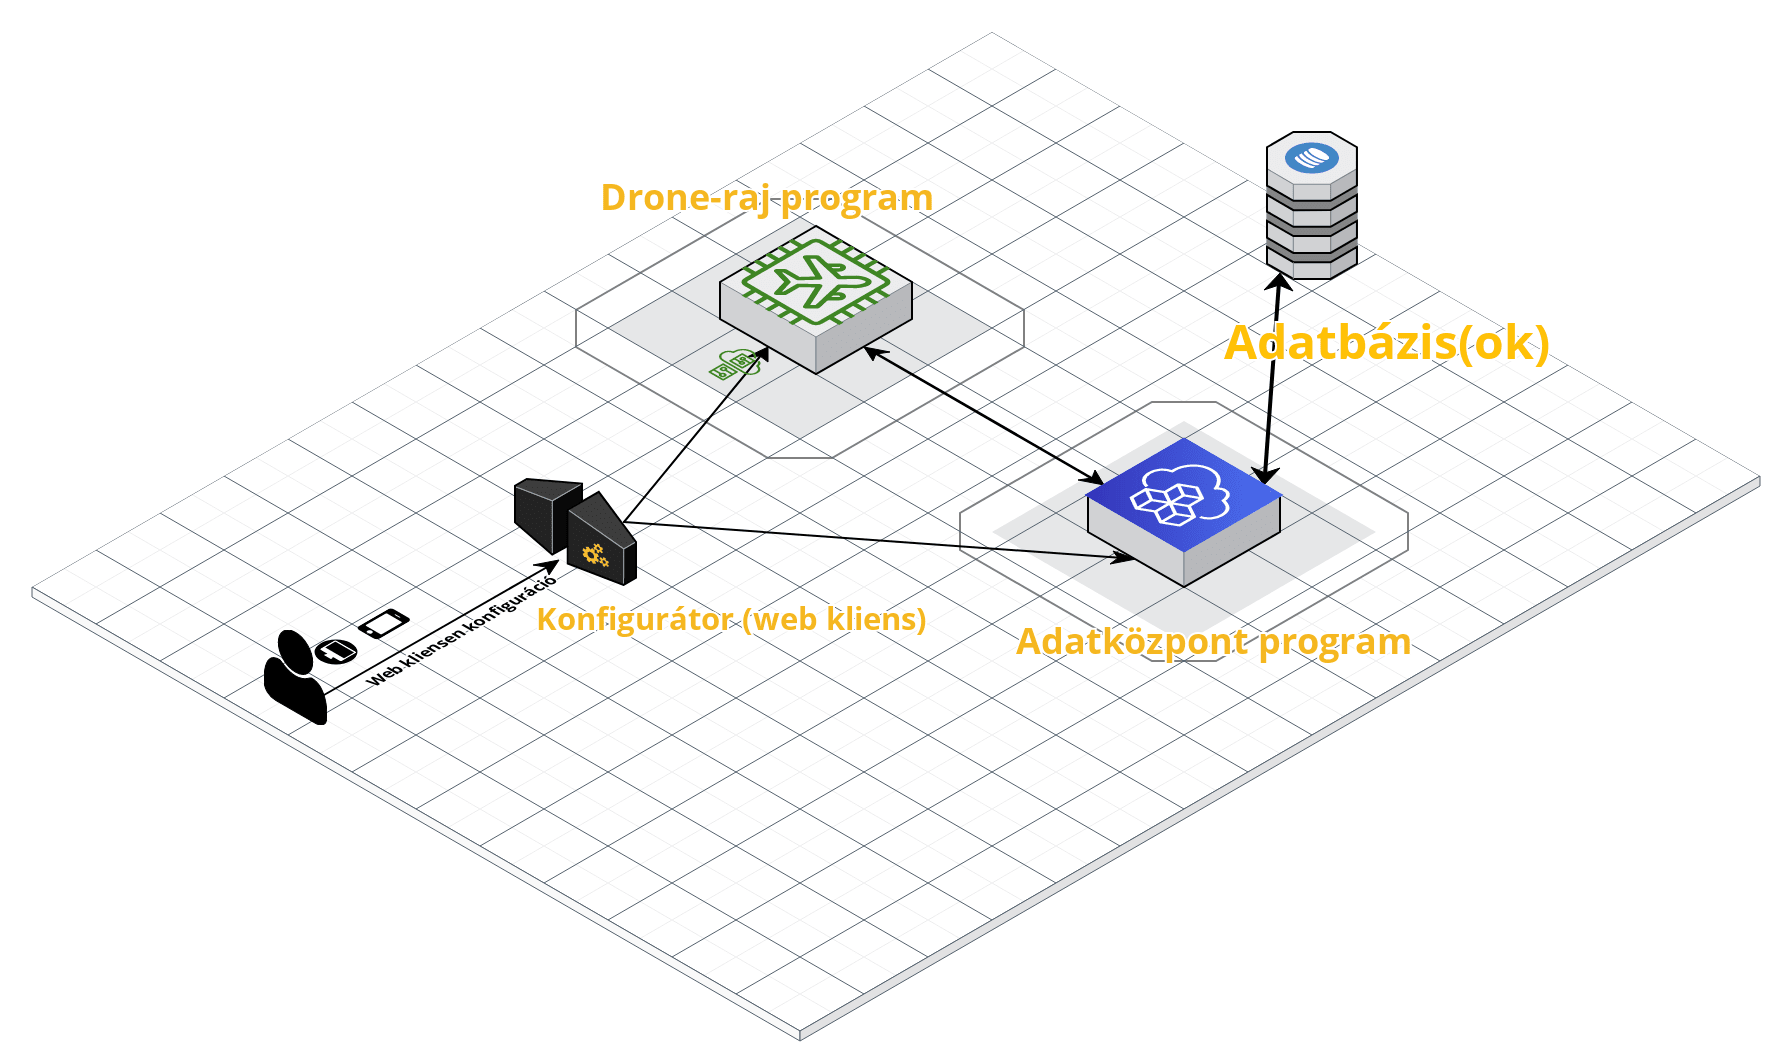
\includegraphics[scale=0.22]{images/szakdolgozat-3-program-abra.png}
    \caption{A 3 program}
    \label{fig:3program}
\end{figure}

\newpage
A szimulációban több féle protokolt és adattovábbításra képes formátumot hasonlítunk össze, így a programot úgy kell felépíteni,
hogy ki lehessen cserélni ezeket a végpontokat anélkül hogy a program üzleti logikájának működését befolyásolnánk.
Az adatközpontok és drónok közötti telemetria adat kommunikációt és annak feldolgozását összehasonlítjuk
egy HTTP 1.1 -en műkodő JSON adatformátumot használó REST \cite{Wikipedia-REST} API-n, egy HTTP 2 -n futó gRPC-t használó végponton is.

\subsection{REST architektúra}

A REST (Representational State Transfer) egy szoftverarchitektúra típus internet alapú rendszerek számára.
Egy REST architektúrának meg kell felelni a következő megszorításoknak:
\begin{itemize}
    \item Kliens-szerver architektúra
    \item Állapotmentesség
    \item Gyorsítótárazhatóság
    \item Réteges felépítés
    \item Egységes interfész
\end{itemize}
Ha ezeket a megkötéseket teljesíti a webes szolgáltatásunk, azt mondhatjuk hogy "RESTful".

\paragraph{Működése}
A kliensek kéréseket indítanak a szerverek felé, a szerverek pedig feldolgozzák a kéréseket és egy választ küldenek vissza.
A kérések és a válaszok erőforrás reprezentációk köré épülnek.
Ezek az erőforrás reprezentációk a mi esetünkben JSON dokumentumok.
Az erőforrásokat az URL címével és a HTTP metódussal azonosítjuk.
A következő példában láthatjuk ahogy egy PUT metódussal és az URL-ben megadott paraméterrel pontosan tudjuk azonosítani mit szeretnénk.
A PUT requestet akkor használjuk ha egy már meglévő erőforrást szeretnénk felülírni, esetünkben az adatbázis konfigurációt kicseréljük.
A :name paraméter pedig megnevezi az erőforrást amire a meglévőt ki szeretnénk cserélni.
Válaszként egy JSON dokumentumot küldünk vissza válaszként a megfelelő státuszkóddal, hogy a kérés sikeres volt vagy sem.

\begin{python}
    router.PUT("/configure/database/:name", func(c echo.Context) error {
        switch c.Param("name") {
            case "mongodb":
            t.ChangeService(m)
            d.ChangeService(m)
            case "postgres":
            t.ChangeService(p)
            d.ChangeService(p)
            default:
            return echo.NewHTTPError(
                http.StatusBadRequest,
                "no such database supported"
            )
        }
        return c.JSON(http.StatusOK, "configuration complete")
    })
\end{python}


\subsection{HTTP/2 gRPC összehasonlítása HTTP/1.1 JSON üzenetváltással}

\paragraph{REST és HTTP 1.1, JSON üzenetváltás}
A mikroszevízes infrastuktúra egy nagyon elterjedt módja az elosztott rendszerek tervezésének.
Sok mikroszervíz a mai napig REST API-n kommunikál, HTTP 1.1-es protokollon keresztül és JSON dokumentumokat küldenek és fogadnak.
Ez a megoldás a fejlesztőknek kedvez, nagyon egyszerű így fejleszteni manapság, rengeteg eszköz van hogy megyorsítsa és megkönnyítse a munkánkat.
De ez a megoldás a teljesítmény rovására megy, ugyanis a következő problémák adódnak vele:
\begin{itemize}
    \item A HTTP/1.1  szöveg alapú és nagyon "nehéz". A kommunikáció hatalmas adatmennyiséget igényel, ez egy felesleges teher.
    \item A HTTP/1.1  állapotmentes, ezért az állapotokat csak a fejlécben tudjuk jelezni, ami nem tömörített.
    \item A HTTP/1.1  unáris - azaz - egy kérésre egy választ kapsz. Nem lehet egyszerre több kérdést küldeni, minden kérésre pontosan egy válasz jön.
    \item Minden egyes HTTP/1.1 kéréshez 3 irányú üzenet váltáshoz van szükség, csak hogy létrehozzuk a TCP kapcsolatot, mivel a TCP kapcsolat full duplex, és mindkét fél szinkronizálja és nyugtázza egymást.
\end{itemize}
Ebből arra következtetünk, hogy olyan szerver és szerver közötti kommunikációra ahol viszonylag sok apró kérés van, vagy a fenti problémák
akadályozzák a programunk működését, akkor érdemes más megoldások után néznünk.

\subsection{RPC}
Az RPC \cite{RPC} (Remote Procedure Call) egy szabvány, olyan távoli eljárás hívás amelynek segítségével használni lehet egy, ugyanabban a hálózatban található távoli gépen futó programot anélkül, hogy a hálózati részletekkel foglalkozni kellene.
Az RPC a kliens/szerver modellt használja (a kérő a kliens, a programot futtató fél a szerver).

\subsection{gRPC}
A gRPC \cite{gRPC} egy Google által fejlesztett RPC keretrendszer, főleg mikroszervizek közötti kommunikációra.
A gRPC HTTP/2-t használ és Protocol Buffert az üzenetváltáshoz JSON helyett. Ez szembemegy a megszokott mikroszervizes architektúra stílussal ami REST-re épül JSON üzenetváltásal HTTP/1.1-en.
Triviális, hogy a legfontosabb előnye az, hogy HTTP/2-n fut és az üzenetváltás Protocol Bufferekkel történik így sokkal gyorsabb és hatékonyabb.


\paragraph{HTTP/1.1 és HTTP/2 összehasonlítása}
A HTTP/2 egy sokkal hatékonyabb protokoll, a streameléssel elérhetjük azt, hogy az egyik fél több üzenetet is küld, a másik fél viszont csak a kérések legvégén válaszol.
\begin{table}[h]
    \centering
    \caption{HTTP/1.1 és HTTP/2}
    \label{tab:http}
    \begin{tabular}{|c|c|}
        \hline
        HTTP/1.1 & HTTP/2 \\
        \hline
        Szöveges formátum & Bináris formátum \\
        \hline
        Fejléc szöveg, nem tömörített & Tömörített fejléc \\
        \hline
        1 kérés, 1 válasz TCP kapcsolatonként & 1 TCP kapcsolatot újra felhasználunk,\\
         & Unáris kérések,\\
        & Szerver streamelés,\\
        & Kliens streamelés,\\
        & Két-irányú streamelés\\
        \hline
    \end{tabular}
\end{table}

\paragraph{Protocol Buffer és JSON összehasonlítása}

Beláthatjuk, hogy a Protocol Buffer egy sokkal hatékonyabb eszköz üzenetek továbbítására.
Mivel nem szöveges, lehet hogy nehezebb implementálni és debugolni a fejlesztőknek, viszont kevesebb adatforgalommal jár, és a számítógép erőforrásait is kíméli, nem úgy mint a JSON.

\begin{table}[h]
    \centering
    \caption{JSON és Protocol Buffer}
    \label{tab:message-exchange}
    \begin{tabular}{|c|c|}
        \hline
        JSON & Protocol Buffer \\
        \hline
        Nincs szigorú séma definíció & Szigorú séma formátum \\
          vagy típus & és típus biztonság \\
        \hline
        Szöveg alapú & Bináris \\
        \hline
        A szöveg formátum miatt lassú & Bináris formátum miatt gyors\\
        szérializáció és deszérializáció & szérializáció és deszérializáció\\
        CPU és memória intenzív & \\
        \hline
        Adatok manuális konvertálása & Generált kód a protokol buffer séma alapján\\
        \hline
    \end{tabular}
\end{table}

\newpage
\subsection{Adatbázisok}
Az adatok adatbázisba mentése, adatbázisból olvasása közben több probléma merülhet fel, a rendszer konkurrens felépítéséből kiindulva.
Például amikor az épp szabad drónoknak adunk feladatot, lehet hogy 2 vagy több egyede az adatközpont programunknak kiolvassa azt az értéket hogy
a drón nem csinál semmit, az állapota szabad, adhat neki feladatot ha van szállítsra váró csomag. De, az üzleti logika futtatása közben az egyik egyed módosíthatta
az értéket arra hogy már repül, vagy épp csomagot vesz fel. Az ilyen Lost Update problémákkal szemben védelmet ad, ha az adatbázis rendelkezik ACID tulajdonságokkal.
Az ACID tulajdonságok \ref{fig:acid} (atomiság, konzisztencia, izoláció, tartósság) felelősek az adatbázis integritásáért.

\begin{figure}[h]
    \centering
    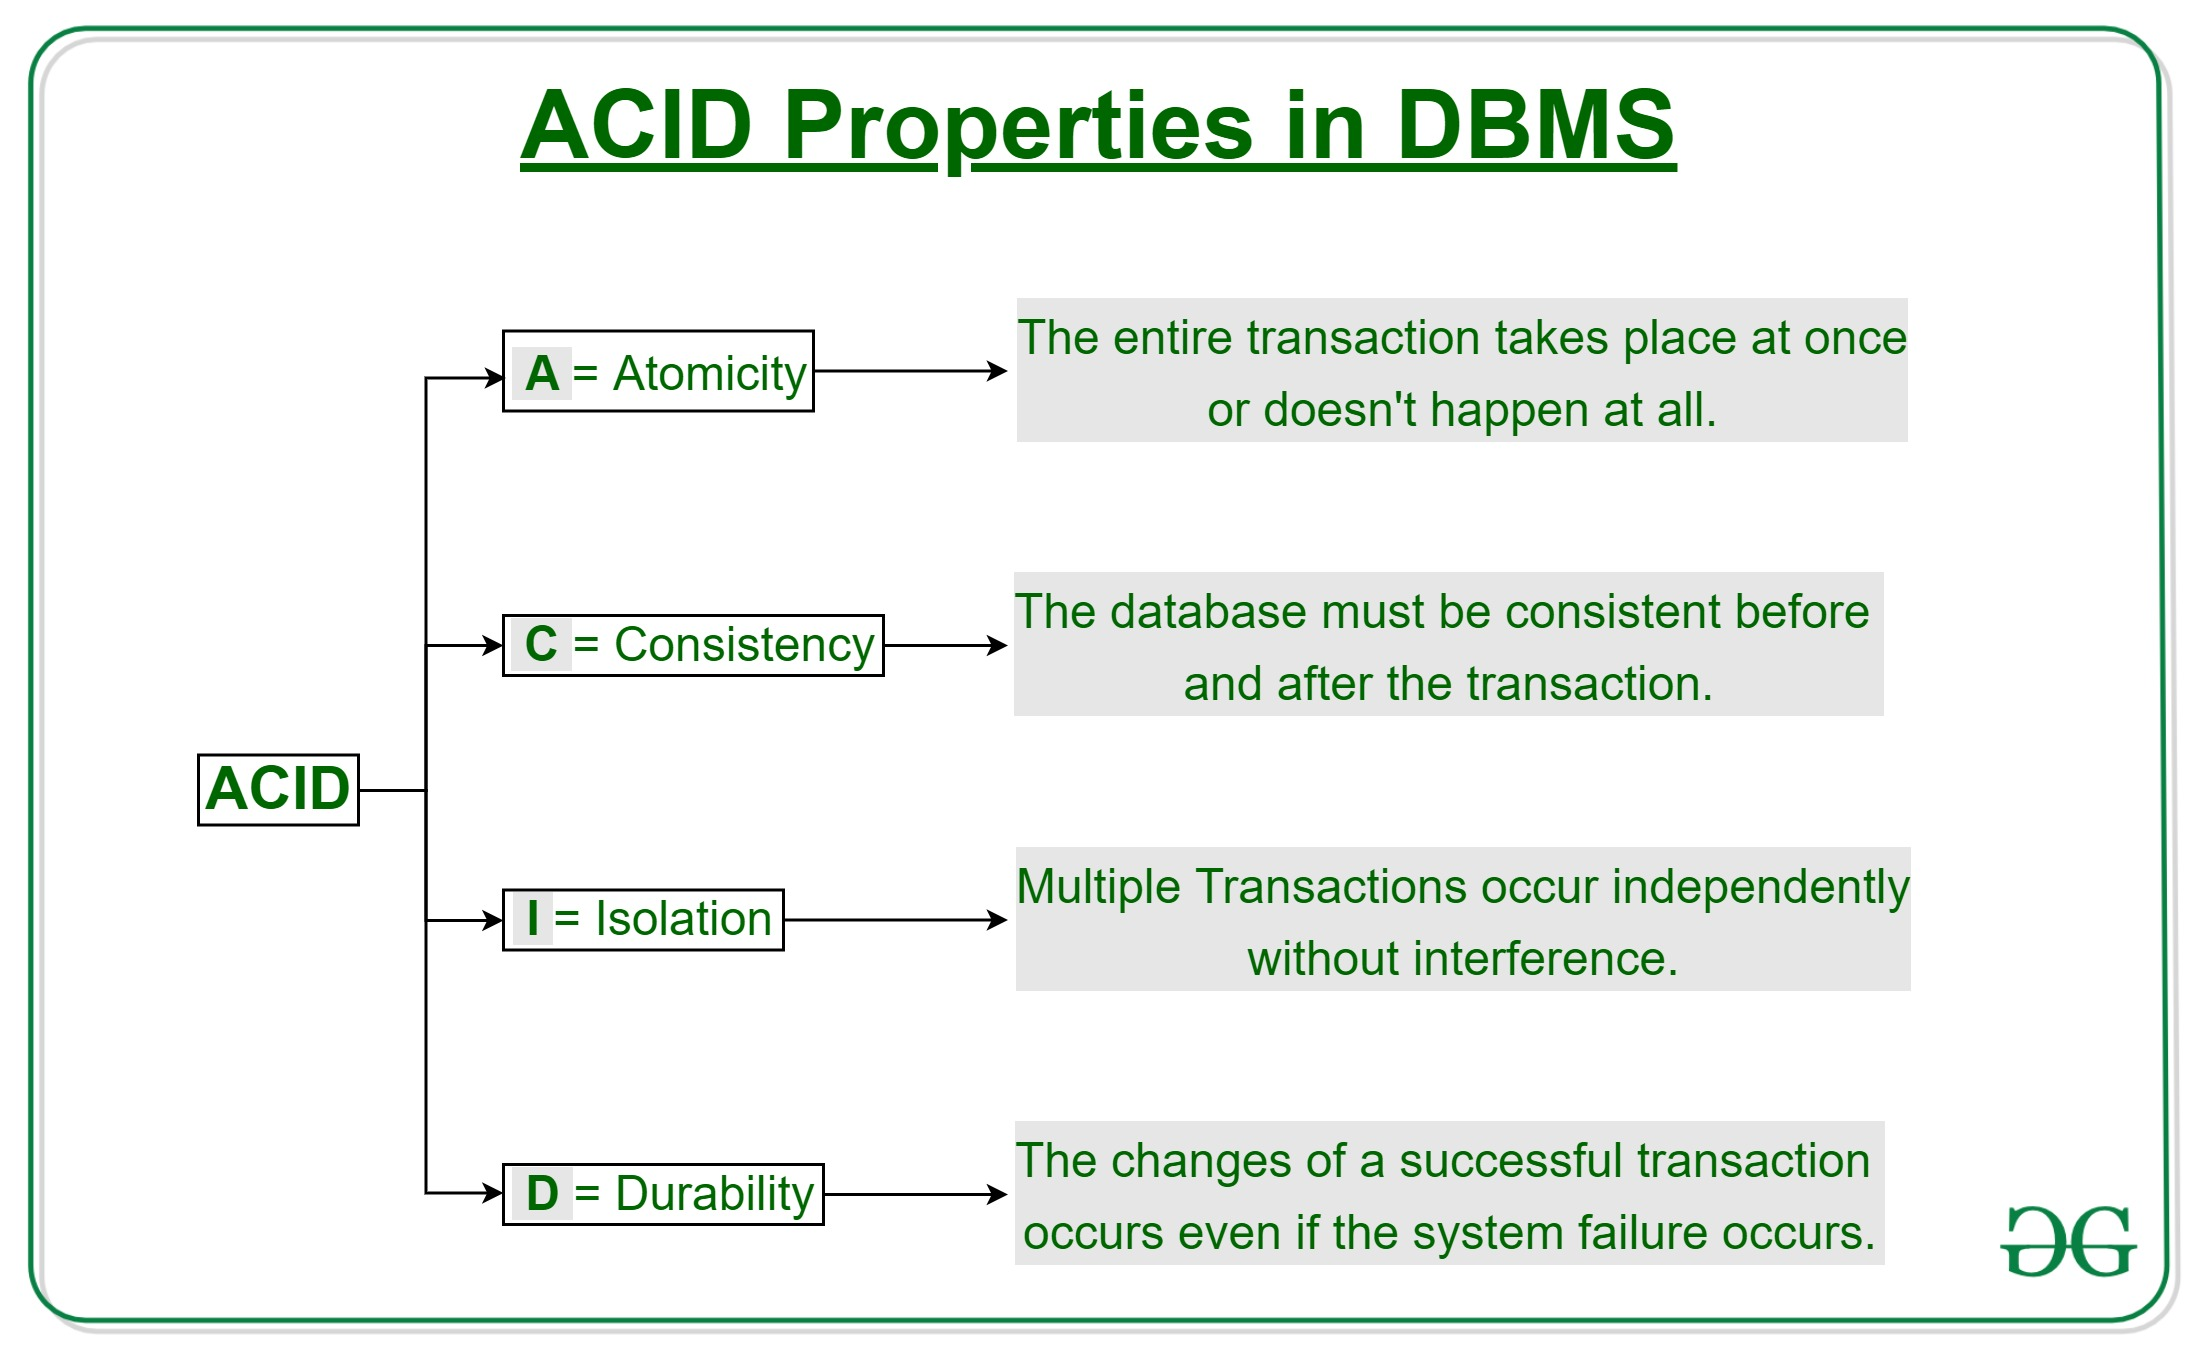
\includegraphics[scale=0.15]{images/ACID-Properties.jpg}
    \caption{ACID tulajdonságok}
    \label{fig:acid}
\end{figure}

Tehát csak olyan adatbázisok jöhetnek szóba a program implementálásánál aminek az integritása garantálható.

\subsection{Protokollok és adatbázisok szerepe a programban}

A drón raj programot és az adatközpontot úgy tervezzük meg, hogy a telemetria adatokat küldéséhez használt rész kicserélhető legyen valamilyen módon (például dependency injekción keresztül).
Így valósítjuk meg a több protokollon keresztüli kommunikációt.
%TODO: ide még írni



%A adatközpont programnak elosztott rendszerként kell működnie, tehát terheléselosztás és megfelelő vezérlés szükséges.
\Section{Program struktúra}
\subsection{Architektúra, program felépítés}
Ahhoz hogy a programot a követelmányben megfogalmazott módon építsük fel, értem ezalatt azt hogy több protokollt és adatbázist hasonlítsunk össze egy olyan
program architektúrát, felépítést kell választani ami megendegi ezt.
Erre a problémára megoldásként a Hexagonal architektúrát \ref{fig:hexagonal-inward} és DDD tervezési alapelvet fogom alkalmazni.
\begin{figure}[h]
    \centering
    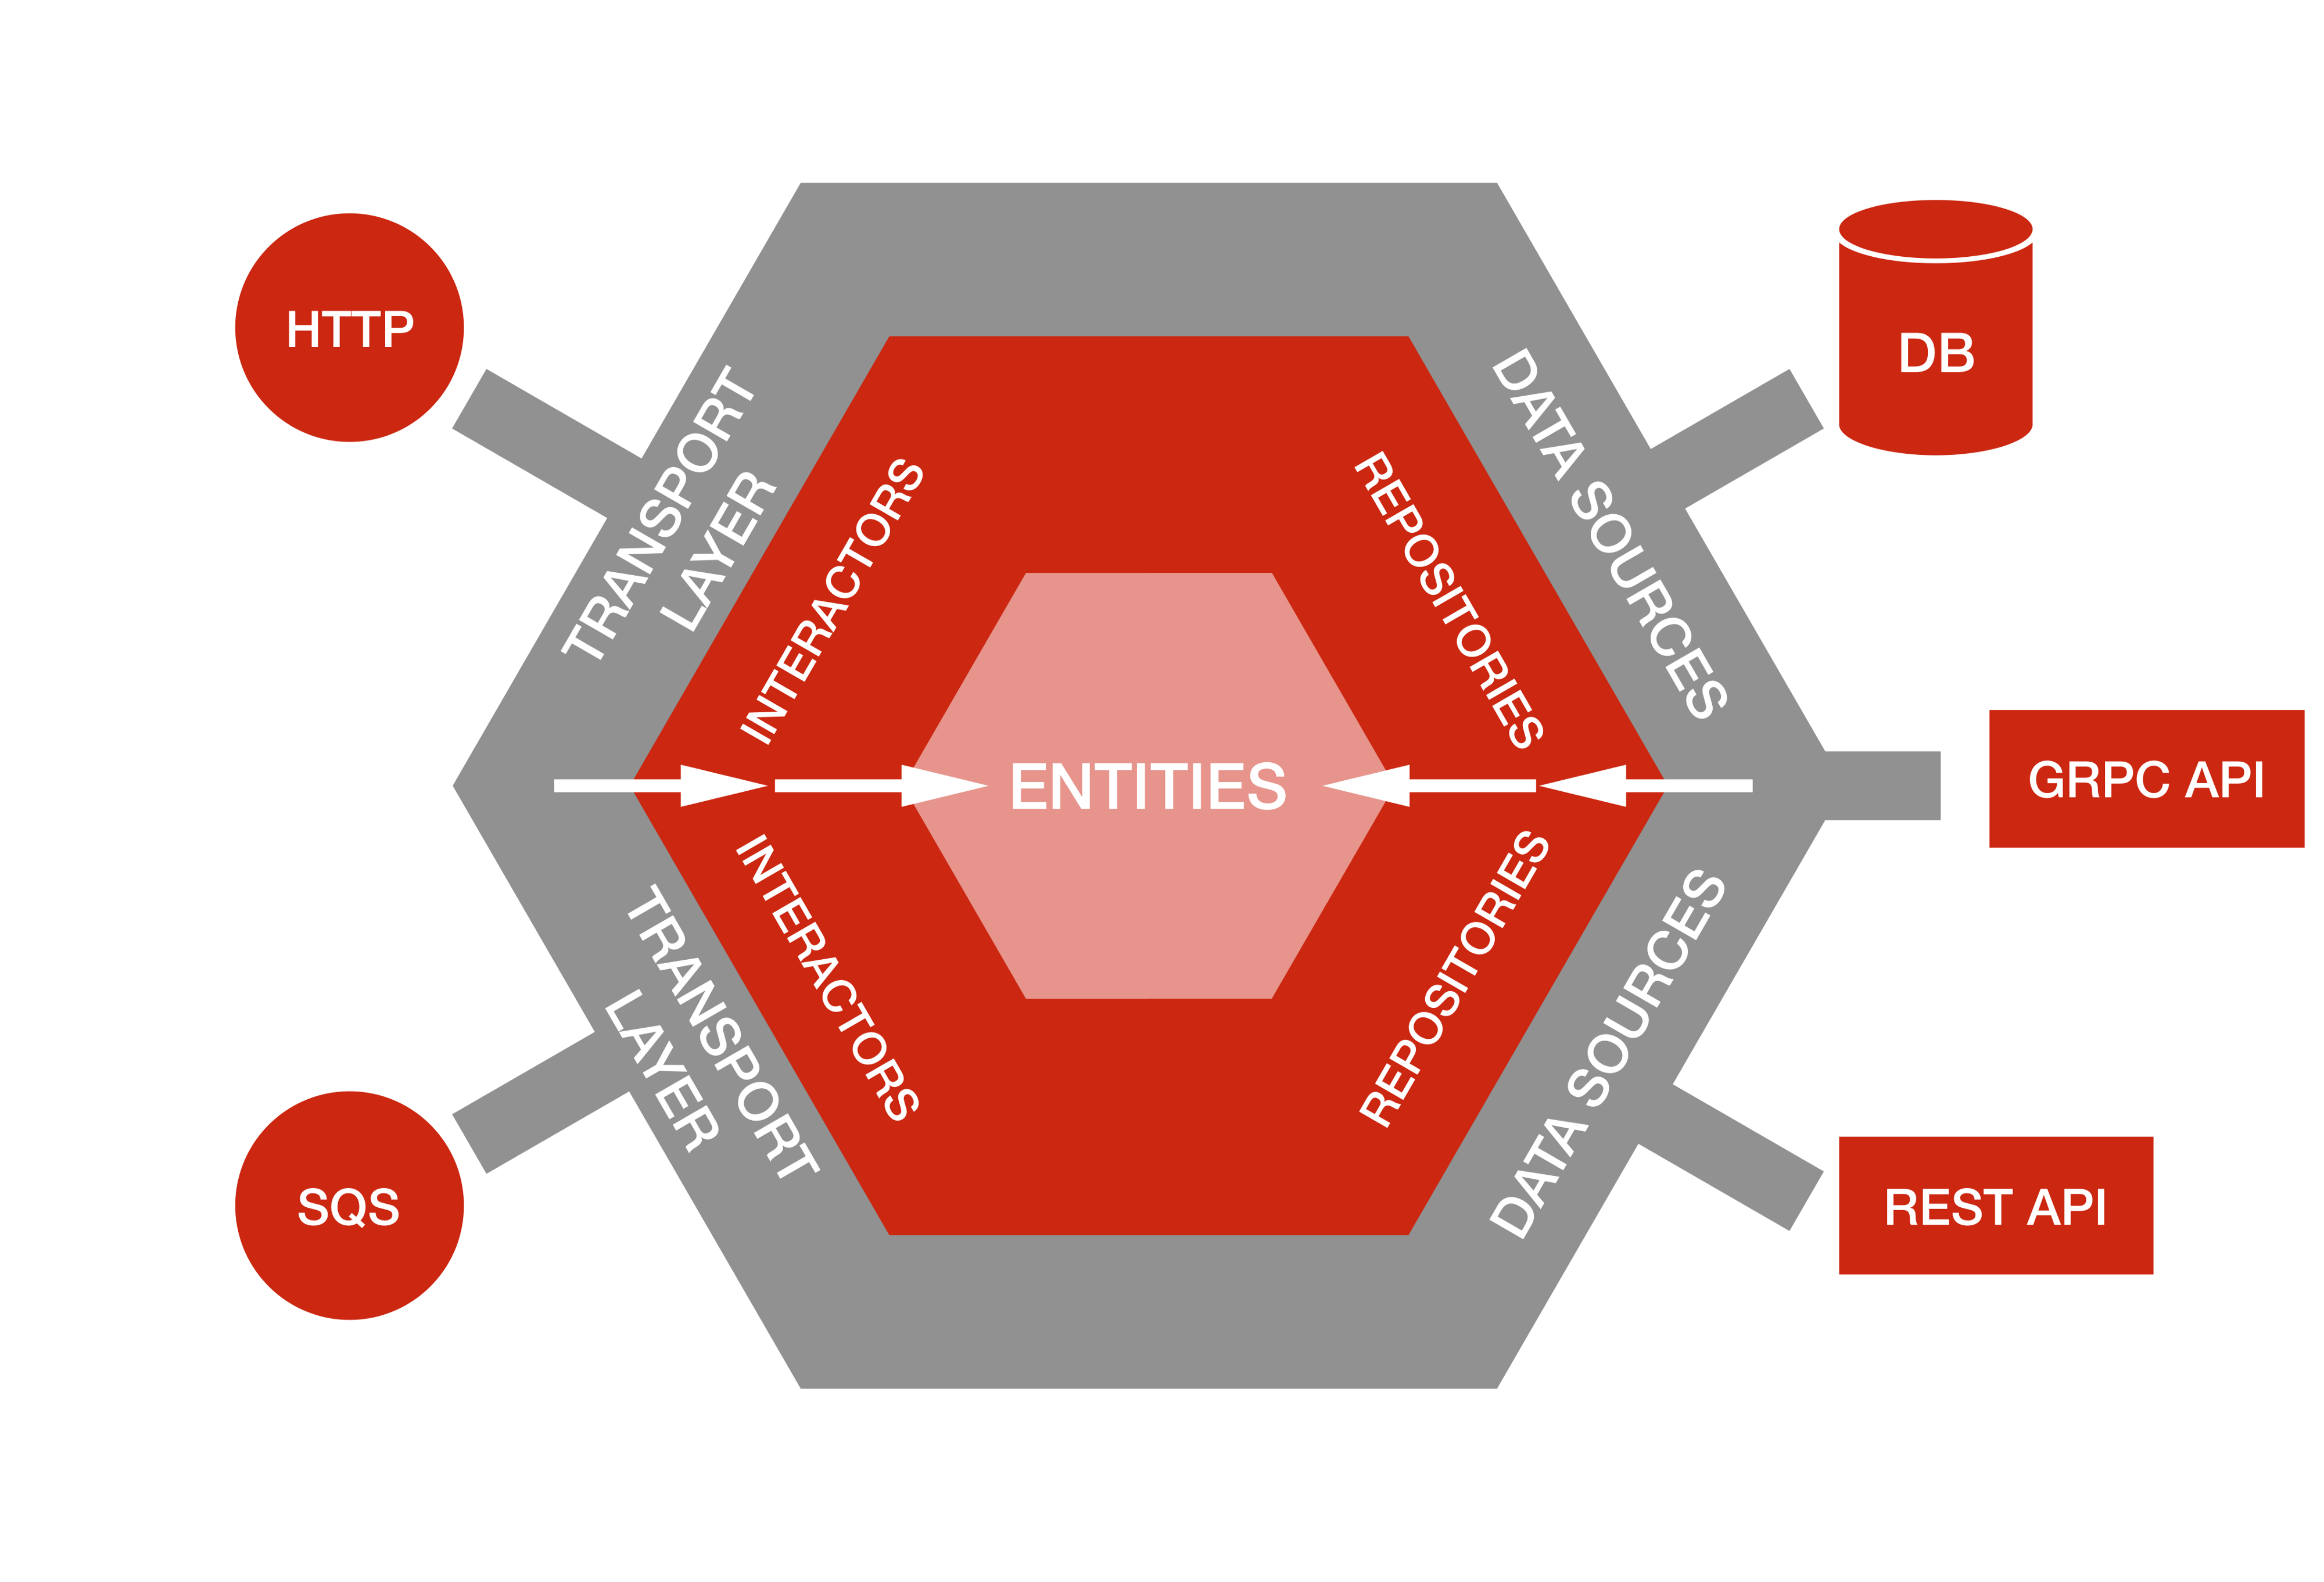
\includegraphics[scale=0.07]{images/hexa-inward.png}
    \caption{Hexagonal architecture inward pointing dependencies}
    \label{fig:hexagonal-inward}
\end{figure}
Így a program belülről kifelé rétegesen epül fel, interfaceket alkalmazva, úgy hogy a pontos implemetáció absztraktálva van, az csak az üzleti logikát ismerjük biztosan, minden ráépülő réteg implementációja cserélhető marad.
Minden réteg csak befelé mutat \ref{fig:hexagonal-inward}, így az üzleti logikánk megmaradhat, miközben az alkalmazás teljes infrastuktúráját kicserélhetnénk.
így a végpontok ha teljesítik az interface elvárásait, csak dependency injection-el kicseréljük a végpontot és minden ugyanúgy működik, ám teljesen más az implementáció.
Azt hogy több fajta input és output végpontot hogy  támogatja az alkalmazás a következő ábra \ref{fig:hexagonal-inward} tökéletesen bemutatja.
Az alkalmazást fel lehet osztani verérlő és vezérelt részre. Ez nagyon jól igazodik az üzleti logikához, egy inputra szinte mindig valamiféle vezérlést várunk el,
tehát hogyha az alkalmazásunkat használjuk, vezéreljük akkor az az adatok hatására valamit csináljon. Ezután az alkalmazásunk beszélhet más, külső forrásokkal, amiket az alkalmazás használ, azaz vezéreli őket.
Ilyen lehet egy adatbázis implementációja, vagy egy üzenet sor, amibe adatokat rakunk be, hogy valami más később kiolvassa.
Azért jó ez a felépítés, mert így például mindegy hogy a terminálból valamilyen konzolos applikáción keresztül hívjuk meg az alkalmazásunkat,
vagy egy webes felületről, esetleg mobil applikációból. A vezérelt egységeket is ki lehet cserélni, nem vagyunk röghöz kötve
mert egyszer így lett megírva az alkalmazésunk, csak a megfelelő réteget kicseréljük, feltéve hogy megírtuk hozzá az implementációnkat és az implementációnk
az intefészen keresztül teljesít minden feltételt. Így például könnyen átállhatunk r1elációs adatbázisról egy dokumentum alapúra, ha valami miatt úgy kívánjuk.
A Netflix is ezt az architektúrát használja \cite{netflix}, ugyanis a gyors növekedésük közben több skálázhatósággal összefüggő problémába ütköztek, amit úgy oldottak meg hogy
ebben az architektúrában\ref{fig:hexagonal-actor} szétosztották a feladatokat több, az adott kis feladatra megfelelő adatbázisra, mikroszervízre.
\begin{figure}[h]
    \centering
    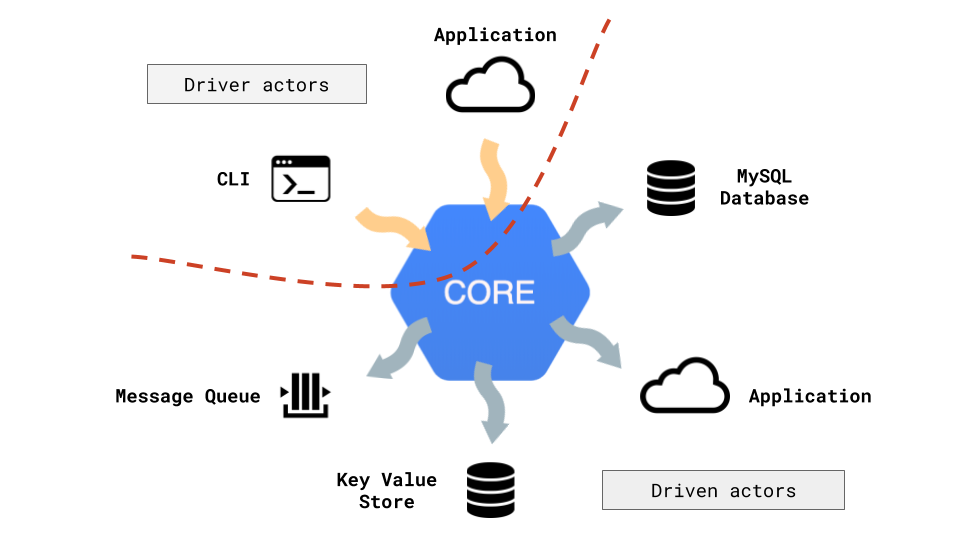
\includegraphics[scale=0.3]{images/hexa-actor.png}
    \caption{Hexagonal architecture driver and driven actors}
    \label{fig:hexagonal-actor}
\end{figure}
\\
A drón-raj program  olyan adatokat fog generálni, amelyet egy valós drónok generálnának és ezeket az adatokat tovább fogja küldeni az adatközpontnak.
%TODO: ide még írni és a program struktúráját jobban megmutatni, a konkrét jegyzék struktúra is akár, hogy mi tartozik infrastruktúrához, mi a program magja stb. Interfacek kapcsolata,
%TODO: Új section ami a program folyamatával foglalkozik, nem a struktúrával



%TODO: Még a struktúrához kell a Go-kit, azért lett ez választva mert nem framework, hanem egy library/ecosystem, így több szabadságot kap a program,
%hogy hogyan is lesz mikroszerviz. Go kit ben van service discovery,  beepitett Observability (Prometheus), többszintes logger, és A hexagonal architektúrát támogatja
%Pl más hasonló mikroszervizeket kezelő framework (pl. Micro) nem elég rugalmas, sok mindent nem enged meg, egy féleképpen lehet használni.



\section{Számítási problémák}

\subsection{Cartesian szerinti}
\begin{gather}
    P_1(5,6,3) \\
    P_2(7,4,9) \\
    V = 10 \frac{m}{s}
\end{gather}


Kiszamitas:

\begin{gather}
    x = r * cos(\phi) * sin(\theta) \\
    y = r * sin(\phi) * sin(\theta) \\
    z = r * cos(\theta)
\end{gather}


X, Y, Z, r

\begin{gather}
    x = X_2 - X_1 = 7 - 5 = 2 \\
    y = Y_2 - Y_1 = 4 - 6 = -2 \\
    z = Z_2 - 7_1 = 9 - 3 = 6 \\
    r = \sqrt{2^2 + (-2)^2 + 6^2} = \sqrt{44}
\end{gather}

$
cos(\phi) sin(\phi) cos(\theta) sin(\theta)
$

\begin{gather}
    cos(\phi) = \frac{x}{\sqrt{x^2 + y^2}} \\
    sin(\phi) = \frac{y}{\sqrt{x^2 + y^2}} \\
    cos(\theta) = \frac{\sqrt(x^2 + y^2)}{\sqrt{x^2 + y^2 + z^2}} \\
    sin(\theta) = \frac{z}{\sqrt{x^2 + y^2 + z^2}}
\end{gather}

\newpage

További számítás segédvektorok kiszámítása:

\begin{gather}
    V_x = \frac{x}{\sqrt{x^2 + y^2 + z^2}} *V = \frac{2}{\sqrt{44}} * 10 = \frac{10\sqrt{11}}{11} = 3.0151\\
    V_y = \frac{y}{\sqrt{x^2 + y^2 + z^2}} *V = \frac{-2}{\sqrt{44}} * 10 = -\frac{10\sqrt{11}}{11} = -3.0151\\\\
    V_z = \frac{z}{\sqrt{x^2 + y^2 + z^2}} *V = \frac{6}{\sqrt{44}} * 10 = \frac{30\sqrt{11}}{11} = 9.0453\\
\end{gather}

Összesen eltelt idő:

\begin{gather}
    t = \frac{s}{v}
\end{gather}

\begin{gather}
    t_osszes = \frac{\sqrt{(x_2 - x_1)^2 + (y_2 - y_1)^2 + (z_2 - z_1)^2}}{v} = \frac{\sqrt{(7 - 5)^2 + (4 - 6)^2 + (9 - 3)^2}}{10} = \frac{\sqrt{44}}{10}{}
\end{gather}

t idő múlva egy adott pillanatban koordináták meghatározása:

\begin{gather}
    x = X_0 + V_x * t = X_0 + \frac{X}{\sqrt{x^2 + y^2 + z^2}} * t = 5 + \frac{2}{\sqrt{44}} * 10 * t \\
    Y = y_0 + V_y * t = y_0 + \frac{y}{\sqrt{x^2 + y^2 + z^2}} * t = 4 - \frac{2}{\sqrt{44}} * 10 * t \\
    z = z_0 + V_z * t = z_0 + \frac{z}{\sqrt{x^2 + y^2 + z^2}} * t = 6 + \frac{6}{\sqrt{44}} * 10 * t
\end{gather}

\subsection{Az Ortodroma számítás, a föld alakját figyelembe véve}

Mivel gömbi geometria lényegesen eltér az euklideszi geometriától ezért a távolságszámításra használt matematikai képletek is eltérőek.
Az euklideszi geometriában a legrövidebb távolságot a két pontot összekötő egyenes,
a nem euklideszi geometriában a két pontot összekötő geodetikus vonal (gömb esetén főkör) mentén mérjük.

\paragraph{A legrövidebb út kiszámítása}
\begin{gather}
    d = arccos(sin\phi_1 * sin\phi_2 * cos\phi_1)* cos\phi_2 * cos\Delta \lambda) * R
\end{gather}

\paragraph{Irány kiszámítása}
Ahogy az főkörön haladunk az irányunk folyamatosan változik. Tehát amikor megérkezünk a célhoz, nem ugyanabban az irányba nézünk mint amikor elindultunk.
A drón szimulációban ez a telemetria adatokban is megfigyelhető.
\begin{gather*}
    \varphi = atan2(sin\Delta\lambda * cos\phi_{2}, cos\phi_{1} * sin\phi_{2} - sin\phi_{1} * cos\phi_{2} * cos\Delta\lambda)
\end{gather*}
ahol $\phi_{1}\lambda_{1}$ a kezdeti pont, és $\phi_{2}\lambda_{2}$ a vég pont és $\Delta\lambda$ pedig a különbség a hosszúsági fokokban.

\paragraph{Cél koordináták kiszámítása, ha ismerjük a megtett távolságot, irányt, és kezdő koordinátákat}
\begin{gather}
    \phi_{2} = arcsin(sin \phi_{1} * cos \delta + cos \phi_{1} * sin \delta * cos \theta)\\
    \lambda_{2} = \lambda_{1} + arctan2(sin\theta * sin\delta  * cos\phi_{1}, cos\delta - sin\phi_{1} * sin\phi_{2})
\end{gather}
ahol $\phi$ a szélességi fok, $\lambda$ a hosszúsági fok, $\theta$ az irány, $\delta$ a szögtávolság d/R és d a megtett távolság, R pedig a Föld sugara.

\Section{Táblázatok}

Táblázatokhoz a \texttt{table} környezetet ajánlott használni.
Erre egy minta \aref{tab:minta}. táblázat.
A hivatkozáshoz az egyedi \texttt{label} értéke konvenció szerint \texttt{tab:} prefixszel kezdődik.

\begin{table}[h]
\centering
\caption{Minta táblázat. A táblázat felirata a táblázat felett kell legyen!}
\label{tab:minta}
\begin{tabular}{l|c|c|}
a & b & c \\
\hline
1 & 2 & 3 \\
4 & 5 & 6 \\
\hline
\end{tabular}
\end{table}

\Section{Ábrák}

Ábrákat a \texttt{figure} környezettel lehet használni.
A használatára egy példa \aref{fig:cimer}. ábrán látható.
Az \texttt{includegraphics} parancsba 
Az ábrák felirata az ábra alatt kell legyen.
Az ábrák hivatkozásához használt nevet konvenció szerint \texttt{fig:}-el célszerű kezdeni.

\begin{figure}[h]
\centering

\includegraphics[scale=0.3]{images/me_logo.png}
\caption{A Miskolci Egyetem címere.}
\label{fig:cimer}
\end{figure}

\Section{További környezetek}

A matematikai témájú dolgozatokban szükség lehet tételek és bizonyításaik megadására.
Ehhez szintén vannak készen elérhető környezetek.

\begin{definition}
Ez egy definíció
\end{definition}

\begin{lemma}
Ez egy lemma
\end{lemma}

\begin{theorem}
Ez egy tétel
\end{theorem}

\begin{proof}
Ez egy bizonyítás
\end{proof}

\begin{corollary}
Ez egy tétel
\end{corollary}

\begin{remark}
Ez egy megjegyzés
\end{remark}

\begin{example}
Ez egy példa
\end{example}

